% =============================================================================
% EXERCISE LIST --- MPE assessment style, graduate level (rules/00_estilo_avaliacao.md §8)
% Aulas 1--2: complementarities (M&R Ch. 1, Ch. 4 pp. 106--113) and
% value maximization / Coase / bargaining (M&R Ch. 2 pp. 35--39; MWG 9.AA)
%
% TWO MODES (one source file):
%   \solucoesfalse  -> blank LIST (space to solve)
%   \solucoestrue   -> ANSWER KEY + RUBRIC
%
% Compile (copyable PDF, global lmodern+cmap rule):
%   pdflatex lista-aulas-01-02.tex   (2x) ; check: pdffonts lista-aulas-01-02.pdf (all Type 1)
% Every result is verified by lista-aulas-01-02-check.py.
% =============================================================================
\documentclass[11pt,a4paper]{article}
\usepackage[utf8]{inputenc}
\usepackage[T1]{fontenc}
\usepackage{lmodern}   % Type 1 vector fonts (replaces PK bitmaps)
\usepackage{cmap}      % ToUnicode CMap -> copyable text and accents
\usepackage[english]{babel}
\usepackage{amsmath,amssymb,amsfonts,mathtools}
\usepackage[a4paper,margin=2.2cm]{geometry}
\usepackage{enumitem}
\usepackage{fancyhdr}
\usepackage{comment}
\usepackage{xcolor}
\usepackage{microtype}
\usepackage{booktabs}
\usepackage{tikz}

% ====================== CONFIGURATION ======================
\newif\ifsolucoes
\solucoesfalse                 % <<<< \solucoestrue for the ANSWER KEY; \solucoesfalse for the LIST

\newcommand{\disciplina}{Economia das Organizações e dos Incentivos --- MPE Insper}
\newcommand{\listatema}{Aulas 1--2: Complementarities, Value Maximization and Bargaining (graduate level)}
\newcommand{\espacoresol}{5cm}   % height of the resolution space in the blank list

% ====================== MACHINERY ======================
\ifsolucoes\includecomment{sol}\else\excludecomment{sol}\fi

\pagestyle{fancy}\fancyhf{}
\lhead{\footnotesize\disciplina}
\rhead{\footnotesize List\ifsolucoes{} --- Answer Key and Rubric\fi}
\cfoot{\footnotesize\thepage}
\renewcommand{\headrulewidth}{0.3pt}
\setlength{\headheight}{14pt}

\setlist{topsep=2pt,itemsep=2pt}
\setlength{\parindent}{0pt}
\newcounter{questao}

\newcommand{\bloco}[3]{\bigskip\noindent
  {\large\bfseries\color{blue!55!black}Block #1 --- #2}\hfill\textit{(#3)}\par
  \noindent\rule{\linewidth}{0.3pt}\smallskip}
\newcommand{\questao}[1]{\refstepcounter{questao}\medskip\noindent
  \textbf{Question \thequestao.}~#1\par}
\newenvironment{alternativas}{\begin{enumerate}[label=\Alph*.,leftmargin=2.2em,topsep=1pt]}{\end{enumerate}}
\newcommand{\gabarito}[1]{\ifsolucoes\par\noindent\textbf{Answer:}~#1\fi}
\newcommand{\resolespaco}{\ifsolucoes\else\par\textit{Resolution:}\vspace{\espacoresol}\par\fi}
\newcommand{\passo}[2]{\par\smallskip\noindent\textbf{Step --- #1.}~#2}
\newcommand{\intuicao}[1]{\par\smallskip\noindent\textit{Economic intuition.}~#1}
\newcommand{\refbib}[1]{\par\smallskip\noindent{\footnotesize\color{black!60}\textbf{Ref:} #1}}
\newcommand{\rubrica}[1]{\par\smallskip\noindent\textbf{Grading rubric.}\begin{itemize}[leftmargin=1.4em,topsep=1pt]#1\end{itemize}}

% =============================================================================
\begin{document}
\begin{center}
  {\Large\bfseries \disciplina}\\[2pt]
  {\large Exercise List: \listatema}\ifsolucoes\\[2pt]\textit{Answer Key and Rubric}\fi
\end{center}
\vspace{2pt}

{\footnotesize\noindent\textbf{Instructions.} Multiple-choice items: mark the single correct
option (no penalty for errors). \emph{True/False} items: every 2 wrong items cancel 1 correct one
(score $=\max\{0,\text{correct}-\text{wrong}/2\}\times$ item value); blank items do not count.
Discursive questions: show every step; a result the item asks you to derive may not be quoted.
All questions are symbolic: state the admissible range of every parameter you use. Throughout,
``quasi-linear'' means $u_i=m_i+(\text{money transfers})+v_i(\cdot)$, i.e.\ no wealth effects in
the sense of Milgrom \& Roberts (1992, p.~35).\par}

% =============================================================================
\bloco{1}{Complementarities and coherent systems}{Aula 1, with Aula 2 \,\textbullet\, 25 points}

\questao{(10 points) Objective items.}

\textbf{a)} (3 points) \emph{Complementarities $\times$ value maximization.} At a Brazilian retail
bank, one director sets the degree of delegation to branch managers, $x$, and another the
intensity of incentive pay, $y$. Bank profit is
$\pi(x,y)=tx+sy+bxy-\tfrac{c_1}{2}x^2-\tfrac{c_2}{2}y^2$, with $b>0$ and $c_1c_2>b^2$. The two
directors have quasi-linear preferences, can sign enforceable agreements on $(x,y)$, make
unrestricted side payments and bargain efficiently. Better local information raises $t$. The
total effect $\mathrm{d}y^*/\mathrm{d}t$ on the agreed incentive intensity is:
\begin{alternativas}
\item $b/(c_1c_2)$
\item $c_2/(c_1c_2-b^2)$
\item $b/(c_1c_2-b^2)$
\item $-b/(c_1c_2+b^2)$
\item $b/(c_2^2-b^2)$
\end{alternativas}
\gabarito{C}
\begin{sol}
\passo{objective}{With quasi-linear preferences and unrestricted transfers, the value maximization
principle makes an agreement efficient iff $(x,y)$ maximizes $\pi$; efficient bargaining (Coase)
therefore selects $\arg\max\pi$ whatever the directors' bargaining power.}
\passo{first-order conditions}{$\pi_x=t+by-c_1x=0$, $\pi_y=s+bx-c_2y=0$; the Hessian
$\begin{psmallmatrix}-c_1&b\\ b&-c_2\end{psmallmatrix}$ is negative definite since $c_1c_2>b^2$.}
\passo{solve}{$x^*=\dfrac{c_2t+bs}{c_1c_2-b^2}$, $y^*=\dfrac{c_1s+bt}{c_1c_2-b^2}$, so
$\dfrac{\mathrm{d}y^*}{\mathrm{d}t}=\dfrac{b}{c_1c_2-b^2}$.}
\passo{distractors}{A stops after one round ($x$ moves $1/c_1$, then $y$ moves $b/c_2$ per unit of
$x$) and ignores the feedback; B is $\mathrm{d}x^*/\mathrm{d}t$; D gets the sign and the
denominator wrong; E applies the symmetric formula $b/(c^2-b^2)$ with the wrong cost.}
\refbib{M\&R Ch.~4, ``Coordination and Business Strategy'', pp.~108--109; Ch.~2, ``The Coase Theorem'', p.~38.}
\end{sol}

\medskip
\textbf{b)} (3 points) A textile firm in Santa Catarina weighs three lean practices
$J,T,S\in\{0,1\}$. Relative to the status quo $(0,0,0)$, profit is
$\pi=-\alpha(J+T+S)+\beta(JT+JS+TS)$ with $\alpha,\beta>0$. The set of parameters for which
(i) adopting all three is the unique global maximum, (ii) every single first step loses money
and (iii) every two-practice corner is below the status quo, is:
\begin{alternativas}
\item $\alpha<\beta<2\alpha$
\item $\beta>\alpha$
\item $\alpha/2<\beta<\alpha$
\item $\beta>2\alpha$
\item $\alpha<\beta<3\alpha$
\end{alternativas}
\gabarito{A}
\begin{sol}
\passo{corners}{By symmetry profit depends on the number $k$ of practices adopted:
$\pi_k=-k\alpha+\beta\binom{k}{2}$, so $\pi_0=0$, $\pi_1=-\alpha$, $\pi_2=-2\alpha+\beta$,
$\pi_3=-3\alpha+3\beta$.}
\passo{conditions}{(i) $\pi_3>\pi_0\Leftrightarrow\beta>\alpha$; then $\pi_3>\pi_1$ and
$\pi_3-\pi_2=2\beta-\alpha>0$ follow. (ii) $\pi_1=-\alpha<0$ holds for every $\alpha>0$: it
imposes nothing. (iii) $\pi_2<0\Leftrightarrow\beta<2\alpha$. Together: $\alpha<\beta<2\alpha$.}
\passo{distractors}{B forgets (iii); D reverses (iii); C reverses (i) and halves the bound;
E takes the bound from $\pi_3$ instead of $\pi_2$.}
\intuicao{In this region every adoption path from Ford's corner to Toyota's falls twice before
it rises: the ``valley'' of Aula 1, created by the complementarity $\beta$ itself.}
\refbib{M\&R Ch.~4, pp.~108--113; Aula 1 notes \S8.1.}
\end{sol}

\medskip
\textbf{c)} (2 points, T or F) \emph{Complementarities $\times$ Coase.} Two managers bargain
efficiently, with quasi-linear preferences and unrestricted transfers, over two
\emph{substitute} practices: $\pi(x,y;t)$ is strictly concave, $\pi_{xy}<0$, $\pi_{xt}>0$ and
$\pi_{yt}=0$. Then the agreed $x$ responds to $t$ by \emph{less} than it would if $y$ were held
fixed.
\gabarito{F}
\begin{sol}
\passo{comparative statics}{Joint maximization (Coase). Differentiating the FOCs:
$\pi_{xx}\,\mathrm{d}x+\pi_{xy}\,\mathrm{d}y=-\pi_{xt}\,\mathrm{d}t$,
$\pi_{xy}\,\mathrm{d}x+\pi_{yy}\,\mathrm{d}y=0$, so
$\dfrac{\mathrm{d}x^*}{\mathrm{d}t}=\dfrac{-\pi_{yy}\pi_{xt}}{\pi_{xx}\pi_{yy}-\pi_{xy}^2}$.
With $y$ fixed, $\mathrm{d}x/\mathrm{d}t=-\pi_{xt}/\pi_{xx}$.}
\passo{ratio}{$\dfrac{\text{total}}{\text{direct}}=\dfrac{\pi_{xx}\pi_{yy}}{\pi_{xx}\pi_{yy}-\pi_{xy}^2}>1$
whenever $\pi_{xy}\neq0$, since strict concavity gives $\pi_{xx}\pi_{yy}>\pi_{xy}^2$. The sign of
$\pi_{xy}$ only decides whether $y$ rises or falls; with substitutes $y$ falls, which raises the
return to $x$ again.}
\refbib{M\&R Ch.~4, p.~108, n.~8; Aula 1 notes \S6.2--6.3.}
\end{sol}

\medskip
\textbf{d)} (2 points, T or F) Let $f(x,t)$ have increasing differences in $(x,t)$ on
$[0,1]\times\mathbb{R}$ and be continuous in $x$. Then the largest maximizer $\bar x(t)$ of
$f(\cdot,t)$ on $[0,1]$ is non-decreasing in $t$, even if $f$ is not concave in $x$.
\gabarito{T}
\begin{sol}
\passo{proof}{Let $t'>t$ and suppose $\bar x'=\bar x(t')<\bar x=\bar x(t)$. Optimality at $t$:
$f(\bar x,t)-f(\bar x',t)\ge0$. Increasing differences: $f(\bar x,t')-f(\bar x',t')\ge
f(\bar x,t)-f(\bar x',t)\ge0$. So $\bar x$ is also a maximizer at $t'$ and $\bar x>\bar x'$,
contradicting that $\bar x'$ is the largest maximizer. No concavity or differentiability is used:
this is Topkis' theorem, the result behind ``complements move together''.}
\refbib{M\&R Ch.~4, p.~108; Milgrom \& Roberts (1990), \emph{AER} 80(3).}
\end{sol}

% -----------------------------------------------------------------------------
\questao{(15 points) \emph{Complementarities (Aula 1) $\times$ value maximization and Coase (Aula 2).}
An auto-parts maker in the ABC paulista is converting a plant to a lean system. There are
$n\ge2$ practices (just-in-time delivery, multi-skilled teams, in-line quality control, \dots),
each run by a different department head; practice $i$ is used at level $x_i\ge0$. Plant profit,
net of all the heads' private costs, is
$$\pi(x)=\sum_{i=1}^n t_ix_i+\frac b2\sum_{i\ne j}x_ix_j-\frac c2\sum_{i=1}^n x_i^2,\qquad t_i>0,\; c>0,\; b\ge0.$$
The heads have quasi-linear preferences, can sign enforceable agreements on every $x_i$, make
unrestricted transfers among themselves, and bargain efficiently. Unless stated otherwise,
$t_i=t$ for all $i$.}

\textbf{a)} (3 points) Explain why the heads choose $x$ to maximize $\pi$ whatever their
bargaining weights. Find the necessary and sufficient condition on $(n,b,c)$ for $\pi$ to have a
unique maximizer, and describe what happens when it fails.
\resolespaco
\begin{sol}
\passo{objective}{Each head $i$ has utility $m_i+\tau_i+v_i(x)$ with $\sum_i\tau_i=0$ (transfers
include the shares of plant revenue), and $\sum_iv_i(x)=\pi(x)$. By the value maximization
principle an agreement is Pareto efficient iff $x\in\arg\max\pi$; efficient bargaining reaches
the Pareto set, and bargaining power only moves the $\tau_i$ (Coase theorem, M\&R p.~38).}
\passo{Hessian}{$\partial^2\pi/\partial x_i^2=-c$, $\partial^2\pi/\partial x_i\partial x_j=b$, so
$H=-(c+b)I+bJ$, with $J$ the all-ones matrix. $J\mathbf 1=n\mathbf 1$ and $Jv=0$ for
$v\perp\mathbf 1$. Eigenvalues: $-(c-(n-1)b)$ on $\mathbf 1$; $-(c+b)$ with multiplicity $n-1$.}
\passo{condition}{$-(c+b)<0$ always. $H$ is negative definite iff $c>(n-1)b$; then $\pi$ is a
strictly concave quadratic, the FOC system is non-singular and has a unique solution, which is
the unique maximizer.}
\passo{failure}{If $c\le(n-1)b$, along the ray $x=\lambda\mathbf 1$:
$\pi=n t\lambda-\tfrac n2(c-(n-1)b)\lambda^2$, which grows without bound as $\lambda\to\infty$
(convex for $c<(n-1)b$, linear with slope $nt>0$ at equality). No maximizer: the plant wants all
practices pushed up together until some capacity bound binds, i.e.\ an all-or-nothing system.}
\intuicao{Each practice's own diminishing returns ($c$) must outweigh the sum of its
complementarities with the other $n-1$ practices; the more practices interlock, the easier it
is for the system to ``run away'' to the extreme.}
\refbib{M\&R Ch.~2, ``The Value Maximization Principle'' and ``The Coase Theorem'', pp.~36--38; Ch.~4, pp.~108--109.}
\rubrica{
\item Value maximization + Coase justification (transfers, quasi-linearity): 1 pt.
\item Eigenvalues of $H$ with eigenvectors: 1 pt; condition $c>(n-1)b$: 0.5 pt.
\item Behaviour when it fails (unbounded along $\mathbf 1$): 0.5 pt.
\item Uses the $n=2$ condition $c>b$ for general $n$: max.\ half the item (special case in the general case).
\item Condition asserted without the eigenvalue (or equivalent) argument: 0 for that line.
}
\end{sol}

\textbf{b)} (3 points) Derive the optimal levels $x^*$ and the maximal profit $\pi^*$. Prove that
the optimum is symmetric.
\resolespaco
\begin{sol}
\passo{FOC}{$\partial\pi/\partial x_i=t+b\sum_{j\ne i}x_j-cx_i=0$ for each $i$.}
\passo{symmetry}{Subtracting the FOCs of $i$ and $k$: $-b(x_i-x_k)-c(x_i-x_k)=0$, i.e.\
$(c+b)(x_i-x_k)=0$, so $x_i=x_k$ since $c+b>0$.}
\passo{level}{With $x_i=\bar x$: $t+(n-1)b\bar x-c\bar x=0$, so
$$x_i^*=\frac{t}{c-(n-1)b}\equiv\frac tD,\qquad D\equiv c-(n-1)b>0.$$}
\passo{value}{$\pi^*=nt\bar x+\tfrac b2n(n-1)\bar x^2-\tfrac c2n\bar x^2=nt\bar x-\tfrac n2D\bar x^2
=\dfrac{n\,t^2}{2D}$. By (a) it is the unique global maximum.}
\refbib{M\&R Ch.~4, p.~108, n.~8.}
\rubrica{
\item FOCs: 0.5 pt; symmetry proved (not assumed): 1 pt.
\item $x^*=t/D$: 1 pt; $\pi^*=nt^2/(2D)$: 0.5 pt; arithmetic slip with the right method: $-0.5$ pt.
\item Symmetry assumed without proof: max.\ 2 pts.
}
\end{sol}

\textbf{c)} (3 points) The return to practice 1 rises ($t_1$ increases, the other $t_i$ fixed).
Derive $\partial x_1^*/\partial t_1$ and $\partial x_j^*/\partial t_1$ for $j\ne1$, and compare
the own response with the response obtained when all other practices are held fixed. For
$n=2$, draw the two best-reply lines in the $(x_1,x_2)$ plane, the optimum before and after the
shock, and the rounds of adjustment in which the two heads take turns re-optimizing.
\resolespaco
\begin{sol}
\passo{linear system}{The FOCs read $((c+b)I-bJ)\,x=t$ (vector of $t_i$). With
$A\equiv(c+b)I-bJ$, Sherman--Morrison gives
$A^{-1}=\dfrac1{c+b}\Big(I+\dfrac{b}{D}J\Big)$ (check: $(c+b)I-bJ$ times it equals $I$ since
$J^2=nJ$ and $c+b-nb=D$). So $\partial x^*/\partial t_1=A^{-1}e_1$.}
\passo{responses}{$$\frac{\partial x_1^*}{\partial t_1}=\frac{1}{c+b}\Big(1+\frac bD\Big)=\frac{c-(n-2)b}{(c+b)D},\qquad
\frac{\partial x_j^*}{\partial t_1}=\frac{b}{(c+b)D}\ge0\quad(j\ne1).$$}
\passo{multiplier}{With the others fixed, $\partial x_1/\partial t_1=1/c$. The ratio is
$$m_n\equiv c\,\frac{\partial x_1^*}{\partial t_1}=\frac{c\,(c-(n-2)b)}{(c+b)(c-(n-1)b)},\qquad m_n-1=\frac{(n-1)b^2}{(c+b)D}>0\ \text{ for } b>0 .$$
For $n=2$: $m_2=c^2/(c^2-b^2)$, Aula 1's multiplier.}
\passo{rounds}{If heads take turns best-responding,
$x^{(k+1)}=\big(t+b(J-I)x^{(k)}\big)/c$. The iteration matrix $(b/c)(J-I)$ has eigenvalues
$(n-1)b/c$ and $-b/c$: the rounds converge iff $(n-1)b<c$, the same condition as in (a). Each
round adds a geometric term, which is why the total exceeds the first-round response $1/c$.}
\passo{graph ($n=2$)}{Best replies $x_1=(t_1+bx_2)/c$ (slope $c/b>1$ in the $(x_1,x_2)$ plane) and
$x_2=(t+bx_1)/c$ (slope $b/c<1$). A rise in $t_1$ shifts head 1's line right by $\Delta t_1/c$; the
staircase alternates horizontal moves (head 1) and vertical moves (head 2) and converges to the new
crossing, up and to the right of the old one.}
\begin{center}
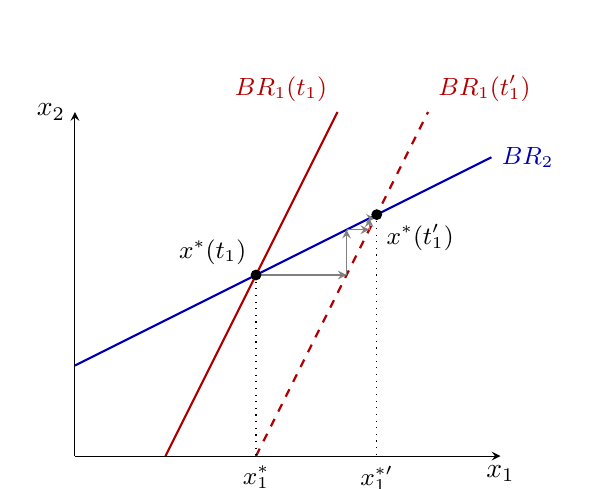
\begin{tikzpicture}[scale=2.3,>=stealth]
  \draw[->] (0,0) -- (2.35,0) node[below] {$x_1$};
  \draw[->] (0,0) -- (0,1.9) node[left] {$x_2$};
  \draw[thick,blue!70!black] (0,0.5) -- (2.3,1.65) node[right] {\small $BR_2$};
  \draw[thick,red!70!black] (0.5,0) -- (1.45,1.9) node[above left] {\small $BR_1(t_1)$};
  \draw[thick,red!70!black,dashed] (1,0) -- (1.95,1.9) node[above right] {\small $BR_1(t_1')$};
  \draw[->,gray] (1,1) -- (1.5,1); \draw[->,gray] (1.5,1) -- (1.5,1.25);
  \draw[->,gray] (1.5,1.25) -- (1.625,1.25); \draw[->,gray] (1.625,1.25) -- (1.625,1.3125);
  \draw[->,gray] (1.625,1.3125) -- (1.656,1.3125);
  \fill (1,1) circle (0.03) node[above left] {\small $x^*(t_1)$};
  \fill (1.6667,1.3333) circle (0.03) node[below right] {\small $x^*(t_1')$};
  \draw[dotted] (1,1) -- (1,0) node[below] {\small $x_1^*$};
  \draw[dotted] (1.6667,1.3333) -- (1.6667,0) node[below] {\small $x_1^{*\prime}$};\end{tikzpicture}
\end{center}
\intuicao{The first round is what a head who ignores the other practices would see ($1/c$). Every
further round is the system's feedback: a higher $x_1$ raises the return to $x_2$, which raises
the return to $x_1$ again (M\&R's ``another round of increases'', p.~108).}
\refbib{M\&R Ch.~4, p.~108, n.~8; Aula 1 notes \S6.2.}
\rubrica{
\item Linear system and its inverse (or Cramer for general $n$): 1 pt.
\item Both derivatives: 0.5 pt; $m_n>1$ proved: 0.5 pt.
\item Graph: labelled axes 0.25, both best replies with correct relative slopes 0.25, shift of
  $BR_1$ 0.25, staircase converging to the new crossing 0.25.
\item Only the $n=2$ formula used for general $n$: max.\ half the item. A graph contradicting the algebra loses the graph points.
}
\end{sol}

\textbf{d)} (3 points) A consultant proposes evaluating the system as $n$ separate pilot
projects: in each pilot one practice is set optimally while all others stay at zero. Define the
\emph{system premium} $P$ as $\pi^*$ minus the sum of the $n$ pilots' profits. Derive $P$ in
closed form, prove that $P>0$ iff $b>0$, and find the share of $\pi^*$ that the pilots miss.
\resolespaco
\begin{sol}
\passo{one pilot}{With $x_j=0$ for $j\ne i$: $\max_{x_i}\,tx_i-\tfrac c2x_i^2$ gives $x_i=t/c$ and
profit $t^2/(2c)$; $n$ pilots sum to $nt^2/(2c)$.}
\passo{premium}{$$P=\frac{nt^2}{2D}-\frac{nt^2}{2c}=\frac{nt^2(c-D)}{2cD}=\frac{n(n-1)\,b\,t^2}{2cD}.$$
Since $D>0$ and $c>0$, $P>0\iff b>0$ (and $P=0$ at $b=0$).}
\passo{share}{$P/\pi^*=1-D/c=(n-1)b/c\in[0,1)$.}
\intuicao{Pilots measure each practice where its complements are absent, which is exactly where
it is worth least. The missing share $(n-1)b/c$ grows with the number of interlocking practices:
this is why GM's practice-by-practice imitation of NUMMI disappointed (Aula 1 notes \S8.2), and
why evidence on single practices understates bundles (Ichniowski, Shaw \& Prennushi 1997).}
\refbib{M\&R Ch.~4, ``Modern Manufacturing Strategy'', pp.~109--110; Ch.~1, pp.~4--6.}
\rubrica{
\item Pilot value $t^2/(2c)$: 1 pt.
\item $P$ in closed form: 1 pt; sign proved: 0.5 pt; share $(n-1)b/c$: 0.5 pt.
\item Pilots computed with the others at $x^*$ instead of zero: max.\ 1 pt (wrong counterfactual).
}
\end{sol}

\textbf{e)} (3 points) Parameter analysis. Prove the sign of the effect of $t$, $b$, $c$ and $n$
(treated as continuous) on $x_i^*$, on profit per practice $\pi^*/n$, on the multiplier $m_n$ and
on the share $P/\pi^*$. Summarize in a table, study the limits $b\to0$ and $(n-1)b\to c^-$, and
give the economic reading.
\resolespaco
\begin{sol}
\passo{levels}{$x^*=t/D$, $\pi^*/n=t^2/(2D)$ with $D=c-(n-1)b$: $\partial D/\partial b=-(n-1)<0$,
$\partial D/\partial n=-b\le0$, $\partial D/\partial c=1$. Both are increasing in $t$, in $b$ and in
$n$, decreasing in $c$ (e.g.\ $\partial x^*/\partial b=t(n-1)/D^2>0$).}
\passo{multiplier}{$m_n=\frac{c}{c+b}\big(1+\frac bD\big)$. In $n$: $D$ falls, so $m_n$ rises.
In $b$:
$$\frac{\partial m_n}{\partial b}=\frac{c\,(n-1)\,b\,(2c-(n-2)b)}{[(c+b)D]^2}>0\quad\text{for } b>0,$$
because $c>(n-1)b$ implies $2c>(n-2)b$. In $c$: $m_n$ is homogeneous of degree 0 in $(b,c)$, so
by Euler $c\,\partial_cm_n+b\,\partial_bm_n=0$ and $\partial_cm_n=-(b/c)\,\partial_bm_n<0$. In $t$: none.}
\passo{share}{$P/\pi^*=(n-1)b/c$: $+$ in $b$ and $n$, $-$ in $c$, $0$ in $t$.}
\begin{center}
\begin{tabular}{lcccc}\toprule
 & $t$ & $b$ & $c$ & $n$\\\midrule
$x_i^*$ & $+$ & $+$ & $-$ & $+$\\
$\pi^*/n$ & $+$ & $+$ & $-$ & $+$\\
$m_n$ & $0$ & $+$ & $-$ & $+$\\
$P/\pi^*$ & $0$ & $+$ & $-$ & $+$\\\bottomrule
\end{tabular}
\end{center}
\passo{limits}{$b\to0$: $x^*=t/c$, $m_n=1$, $P=0$; practices are independent and piecemeal
evaluation is exact. $(n-1)b\to c^-$: $D\to0^+$, so $x^*$, $\pi^*$, $m_n\to\infty$ and
$P/\pi^*\to1$; almost all value is systemic. Beyond it, (a) shows there is no interior optimum.
$n=1$: $m_1=1$.}
\passo{reading}{Stronger or more numerous complementarities make the system both more valuable
and more sensitive: a small change in one practice's return moves every practice, and isolated
trials see an ever smaller part of the value. Near the knife edge, a plant's choice becomes
all-or-nothing, the coherent-systems logic of M\&R Figure 4.3 (p.~111).}
\rubrica{
\item Signs of $x^*$ and $\pi^*/n$ proved: 1 pt. Multiplier signs proved (incl.\ the $c$ sign): 1 pt.
\item Table: 0.25 pt; limits: 0.25 pt; economic reading: 0.5 pt.
\item Signs listed without proof or reading: max.\ half the item. A sign claim without proof: 0 for that line.
}
\end{sol}

% =============================================================================
\bloco{2}{Value maximization, the Coase theorem and the division of surplus}{Aula 2 \,\textbullet\, 25 points}

\questao{(10 points) Objective items.}

\textbf{a)} (3 points) A Petrobras technician chooses between two shift assignments $y_1,y_2$
(M\&R's overtime example, p.~38); $x>0$ is money and $v(\cdot)$ is a real-valued function.
Ignoring the ability-to-pay condition (wealth is large), which utility function displays
\emph{no wealth effects} in M\&R's sense (p.~35)?
\begin{alternativas}
\item $u(x,y)=\ln x+v(y)$
\item $u(x,y)=x\,e^{v(y)}$
\item $u(x,y)=x+v(y)\sqrt x$
\item $u(x,y)=\big(x+v(y)\big)^3$
\item $u(x,y)=v(y)\ln x$, with $v>0$
\end{alternativas}
\gabarito{D}
\begin{sol}
\passo{test}{No wealth effects $\Leftrightarrow$ the compensation $\Delta$ for switching
$y_1\to y_2$, defined by $u(M+\Delta,y_2)=u(M,y_1)$, exists and does not depend on $M$.}
\passo{options}{A, B: $\Delta=M(e^{v(y_1)-v(y_2)}-1)$, proportional to $M$. C: $\Delta$ solves
$M+\Delta+v_2\sqrt{M+\Delta}=M+v_1\sqrt M$, which depends on $M$. E: $\Delta=M^{v_1/v_2}-M$.
D: $z\mapsto z^3$ is strictly increasing, so $u(M+\Delta,y_2)=u(M,y_1)\iff
M+\Delta+v_2=M+v_1\iff\Delta=v_1-v_2$, independent of $M$.}
\intuicao{``No wealth effects'' is a property of preferences, not of one utility function: any
increasing transformation of $x+v(y)$ represents the same preferences (the logic of M\&R
Mathematical Exercise 2.4, p.~53). The trap is to look for the literal form $x+v(y)$.}
\refbib{M\&R Ch.~2, ``The Value Maximization Principle'', pp.~35--36 and n.~7.}
\end{sol}

\medskip
\textbf{b)} (3 points) In Cubatão (SP) a chemical plant gains $G>0$ from discharging effluent
into a river; the neighbourhood downstream, with wealth $M$, has utility
$u=2\sqrt x+\theta c$, where $c\in\{0,1\}$ indicates a clean river and $0<\theta<2\sqrt M$.
Bargaining is costless and information complete. The set of values of $G$ for which the
assignment of the right (to the plant or to the neighbourhood) decides whether discharging
occurs is:
\begin{alternativas}
\item empty (the Coase theorem applies whatever the utility function)
\item $\big(\theta\sqrt M-\theta^2/4,\ \theta\sqrt M+\theta^2/4\big)$
\item $\big(\theta\sqrt M-\theta^2/2,\ \theta\sqrt M+\theta^2/2\big)$
\item $\big(\theta\sqrt M,\ \theta\sqrt M+\theta^2/4\big)$
\item $\big(2\theta\sqrt M-\theta^2/2,\ 2\theta\sqrt M+\theta^2/2\big)$
\end{alternativas}
\gabarito{B}
\begin{sol}
\passo{WTP}{Plant holds the right; residents pay at most $p$:
$2\sqrt{M-p}+\theta=2\sqrt M\Rightarrow p=M-(\sqrt M-\theta/2)^2=\theta\sqrt M-\theta^2/4$
(admissible since $\theta<2\sqrt M$).}
\passo{WTA}{Residents hold the right; they accept no less than $a$:
$2\sqrt{M+a}=2\sqrt M+\theta\Rightarrow a=\theta\sqrt M+\theta^2/4$.}
\passo{outcomes}{Plant's right: discharge unless residents pay more than $G$, i.e.\ discharge iff
$G>p$. Residents' right: discharge iff $G>a$. The assignment matters iff $p<G<a$: option B. The
interval has width $a-p=\theta^2/2>0$: the wealth effect. With quasi-linear $u=x+\theta c$, $p=a$
and the set is empty (A's claim is the Coase theorem used outside its hypotheses).}
\refbib{M\&R Ch.~2, ``The Coase Theorem'', p.~38, and n.~10, p.~37; Cabral (2017) \S5.1, pp.~97--98.}
\end{sol}

\medskip
\textbf{c)} (2 points, T or F) \emph{Coase $\times$ complementarities.} Two divisions with
quasi-linear preferences control complementary practices: division 1 sets $x$, division 2 sets
$y$, joint profit $\pi=tx+sy+bxy-\tfrac{c_1}2x^2-\tfrac{c_2}2y^2$ with $t,s,b>0$,
$c_1c_2>b^2$. They contract on $(x,y)$ with unrestricted transfers and bargain efficiently. A
rise in division 1's cost parameter $c_1$ lowers the agreed level of $y$.
\gabarito{T}
\begin{sol}
\passo{proof}{By Coase they maximize $\pi$, so $y^*=\dfrac{c_1s+bt}{c_1c_2-b^2}$ and
$$\frac{\partial y^*}{\partial c_1}=\frac{s(c_1c_2-b^2)-c_2(c_1s+bt)}{(c_1c_2-b^2)^2}
=-\frac{b\,(bs+c_2t)}{(c_1c_2-b^2)^2}<0.$$}
\intuicao{Which division bears the cost does not matter for the agreed plan (only for the
transfer); what matters is that $x$ falls, and $y$, its complement, follows it.}
\refbib{M\&R Ch.~2, p.~38; Ch.~4, p.~108.}
\end{sol}

\medskip
\textbf{d)} (2 points, T or F) \emph{Bargaining $\times$ complementarities.} In the setting of item
c), the agreement is the generalized Nash bargaining solution with weight $\beta\in(0,1)$ for
division 1 and threat points $(d_1,d_2)$. A better outside option for division 1 (higher $d_1$)
raises both agreed levels $x$ and $y$, because complements move together.
\gabarito{F}
\begin{sol}
\passo{proof}{With transferable utility the Nash product
$(u_1-d_1)^\beta(u_2-d_2)^{1-\beta}$, maximized over $u_1+u_2=\pi(x,y)$, equals
$\beta^\beta(1-\beta)^{1-\beta}\,(\pi(x,y)-d_1-d_2)$ at the best split, which is increasing in
$\pi$: the solution picks $\arg\max\pi$, independent of $(d_1,d_2,\beta)$. Only payoffs move:
$u_1=d_1+\beta(\pi^*-d_1-d_2)$, so $\partial u_1/\partial d_1=1-\beta$, through the transfer.
``Complements move together'' applies to parameters that shift marginal returns, and $d_1$
shifts none.}
\refbib{M\&R Ch.~2, ``The Coase Theorem'', p.~38; Varian (2014, with Calculus) \S30.7, p.~581.}
\end{sol}

% -----------------------------------------------------------------------------
\questao{(15 points) \emph{Bargaining (Nash solution, threat points) $\times$ efficiency (value
maximization, wealth effects).} On a river of the São Francisco basin, an irrigation company $U$
upstream chooses its withdrawal $y\ge0$; a fishing cooperative $D$ downstream is harmed. $U$'s
gross benefit is $B(y)=\alpha y-\tfrac12y^2$; $D$'s harm in money is $\tfrac\kappa2y^2$, with
$\alpha>0$, $\kappa>0$. The water agency (ANA) gives the right either to $D$ (\emph{regime D}: no
withdrawal without $D$'s consent) or to $U$ (\emph{regime U}: unrestricted withdrawal). Both
parties observe $y$ and all parameters, can contract on $y$ and on a transfer, and the agreement
is the generalized Nash bargaining solution with weight $\beta\in(0,1)$ for $U$; each regime's
threat point is the outcome without agreement. Until item d), preferences are
$u_U=m_U+B(y)+x_U$, $u_D=m_D-\tfrac\kappa2y^2+x_D$, with $x_U+x_D=0$.}

\textbf{a)} (3 points) Prove that the Pareto-efficient allocations are exactly those with one
particular withdrawal level, and find it.
\resolespaco
\begin{sol}
\passo{total value}{For any allocation $(y,x_U,x_D)$ with $x_U+x_D=0$:
$u_U+u_D=m_U+m_D+W(y)$, $W(y)\equiv B(y)-\tfrac\kappa2y^2=\alpha y-\tfrac{1+\kappa}2y^2$.
Transfers drop out.}
\passo{if}{Let $y^*\in\arg\max W$. Any feasible pair satisfies $u_U+u_D\le m_U+m_D+W(y^*)$; an
allocation with $y^*$ lies on this line, so raising one utility lowers the other: efficient.}
\passo{only if}{If $W(y)<W(y^*)$, give each party its old utility plus
$\tfrac12[W(y^*)-W(y)]>0$ at $y^*$ (feasible, because transfers are unrestricted): both strictly
gain, so $y$ was inefficient.}
\passo{level}{$W''=-(1+\kappa)<0$; $W'(y)=\alpha-(1+\kappa)y=0\Rightarrow y^*=\dfrac{\alpha}{1+\kappa}$,
$W^*=\dfrac{\alpha^2}{2(1+\kappa)}$.}
\refbib{M\&R Ch.~2, ``The Logic of Value Maximization'', p.~37, Figure 2.1.}
\rubrica{
\item Transfers drop out of the total: 0.5 pt. Both directions of the proof: 1.5 pts.
\item $y^*$ and $W^*$ with the second-order condition: 1 pt.
\item Only one direction proved: max.\ 2 pts. Principle quoted instead of proved: max.\ 1 pt.
}
\end{sol}

\textbf{b)} (3 points) Characterize the bargaining outcome in each regime: threat points,
withdrawal, the transfer (with its direction) and both payoffs. What does the comparison
show?
\resolespaco
\begin{sol}
\passo{Nash with transferable utility}{Payoffs net of $m_i$. For any $y$, feasible pairs satisfy
$u_U+u_D=W(y)$. Maximizing $(u_U-d_U)^\beta(u_D-d_D)^{1-\beta}$ on that line gives gains in
proportion $\beta:(1-\beta)$ and a maximized product $\beta^\beta(1-\beta)^{1-\beta}(W(y)-d_U-d_D)$,
increasing in $W(y)$. Hence $y=y^*$ and $u_U=d_U+\beta S$, $u_D=d_D+(1-\beta)S$, with
$S=W^*-d_U-d_D$.}
\passo{regime D}{Without agreement $y=0$: $(d_U,d_D)=(0,0)$, $S_D=W^*>0$. $U$ pays $D$
$\tau_D$ with $B(y^*)-\tau_D=\beta W^*$. Since $B(y^*)=\dfrac{\alpha^2(1+2\kappa)}{2(1+\kappa)^2}$,
$$\tau_D=\frac{\alpha^2\,[1+2\kappa-\beta(1+\kappa)]}{2(1+\kappa)^2}
=\underbrace{\tfrac\kappa2y^{*2}}_{\text{harm}}+(1-\beta)W^*>0 .$$}
\passo{regime U}{Without agreement $U$ maximizes $B$: $y=\alpha$, $(d_U,d_D)=(\tfrac{\alpha^2}2,-\tfrac{\kappa\alpha^2}2)$.
$S_U=W^*-\tfrac{\alpha^2}{2}(1-\kappa)=\dfrac{\alpha^2\kappa^2}{2(1+\kappa)}>0$. $D$ pays $U$
$\tau_U$ with $B(y^*)+\tau_U=\tfrac{\alpha^2}2+\beta S_U$:
$$\tau_U=\frac{\alpha^2\kappa^2\,[1+\beta(1+\kappa)]}{2(1+\kappa)^2}>0.$$
Payoffs: $u_U=\tfrac{\alpha^2}2+\beta S_U$, $u_D=-\tfrac{\kappa\alpha^2}2+(1-\beta)S_U$.}
\passo{comparison}{$y=y^*$ in both regimes and for every $\beta$: the withdrawal does not depend on
who holds the right or on bargaining power. The regime decides the direction and size of the
transfer and the threat points (Coase theorem).}
\intuicao{The right is an asset: whoever holds it sells part of it to the other side at a price
set by the threat points and $\beta$, and the sale always lands at the value-maximizing withdrawal.}
\refbib{M\&R Ch.~2, ``The Coase Theorem'', p.~38; Cabral (2017) \S5.1, pp.~97--98.}
\rubrica{
\item Nash solution selects $y^*$ (shown, not assumed): 1 pt.
\item Regime D threat points and $\tau_D$: 0.75 pt. Regime U threat points, $S_U$ and $\tau_U$: 0.75 pt.
\item Coase conclusion stated with its hypotheses: 0.5 pt.
\item Threat point in regime U taken as $y=0$: max.\ 1.5 pts. Arithmetic slip with the right method: $-0.5$ pt.
}
\end{sol}

\textbf{c)} (3 points) In the plane of payoffs net of $m_i$, $(u_U,u_D)$, draw the utility
possibility frontier, the threat points of both regimes and both bargaining outcomes. Read the
Coase theorem off the figure.
\resolespaco
\begin{sol}
\passo{figure}{The frontier is the line $u_U+u_D=W^*$ of slope $-1$. Threat points:
$d^D=(0,0)$ below it, $d^U=(\tfrac{\alpha^2}2,-\tfrac{\kappa\alpha^2}2)$ on the lower line
$u_U+u_D=\tfrac{\alpha^2}2(1-\kappa)$. Each outcome is reached from its threat point by moving
onto the frontier, $U$ taking the fraction $\beta$ of the gap (drawn with $\beta=\tfrac12$:
$45^\circ$ moves).}
\begin{center}
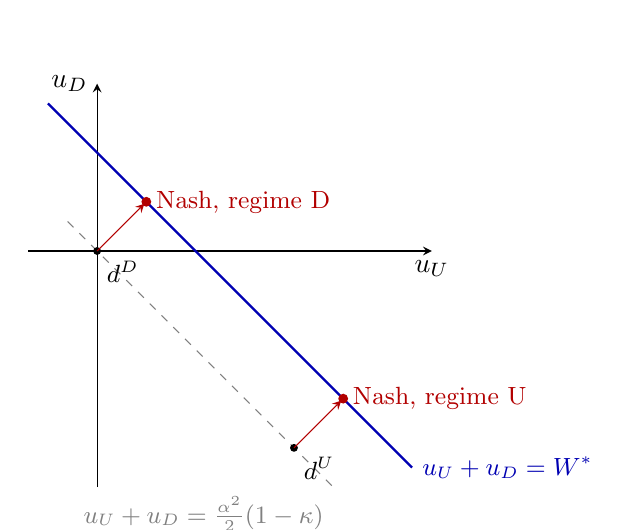
\begin{tikzpicture}[scale=1.25,>=stealth]
  \draw[->] (-0.7,0) -- (3.4,0) node[below] {$u_U$};
  \draw[->] (0,-2.4) -- (0,1.7) node[left] {$u_D$};
  \draw[thick,blue!70!black] (-0.5,1.5) -- (3.2,-2.2) node[right] {\small $u_U+u_D=W^*$};
  \draw[dashed,gray] (-0.3,0.3) -- (2.4,-2.4) node[below left] {\small $u_U+u_D=\tfrac{\alpha^2}{2}(1-\kappa)$};
  \fill (0,0) circle (0.04) node[below right] {\small $d^D$};
  \fill (2,-2) circle (0.04) node[below right] {\small $d^U$};
  \draw[->,red!70!black] (0,0) -- (0.48,0.48);
  \fill[red!70!black] (0.5,0.5) circle (0.05) node[right] {\small Nash, regime D};
  \draw[->,red!70!black] (2,-2) -- (2.48,-1.52);
  \fill[red!70!black] (2.5,-1.5) circle (0.05) node[right] {\small Nash, regime U};
\end{tikzpicture}
\end{center}
\passo{reading}{Both outcomes lie on the same frontier, which is generated by the single
withdrawal $y^*$: the regime moves the outcome \emph{along} the frontier (distribution), never
off it (efficiency). With wealth effects the frontier would be curved, and points on it would
correspond to different $y$ (item d).}
\refbib{M\&R Ch.~2, Figure 2.1, p.~37.}
\rubrica{
\item Labelled axes: 0.5 pt. Frontier of slope $-1$ at $W^*$: 0.5 pt.
\item Both threat points correctly placed (incl.\ $d^U$ below the frontier): 0.75 pt.
\item Both outcomes on the frontier, reached in proportion $\beta$: 0.75 pt. Reading: 0.5 pt.
\item A figure that contradicts the student's algebra loses the figure points.
}
\end{sol}

\textbf{d)} (3 points) Now $D$'s utility is $h(m_D+x_D)-\tfrac\kappa2y^2$, with $h'>0$, $h''<0$
($U$ unchanged). Characterize the Pareto frontier: show that along it the efficient withdrawal is
a strictly decreasing function of $D$'s utility, and give the case $h(w)=\ln w$. Use this to
show that, if every agreement $U$ accepts in regime U leaves $D$ worse off than $h(m_D)$, then
every agreement of regime U has a strictly larger withdrawal than every agreement of regime D.
Which special case of $h$ restores item a)?
\resolespaco
\begin{sol}
\passo{problem}{Let $w\equiv m_D+x_D$ be $D$'s final wealth. Frontier: maximize
$m_U+B(y)-x_D$ subject to $h(m_D+x_D)-\tfrac\kappa2y^2\ge\bar u_D$. Lagrangian with multiplier
$\lambda$ (the value to $U$ of a unit of $D$'s utility).}
\passo{FOCs}{$x_D$: $-1+\lambda h'(w)=0\Rightarrow\lambda=1/h'(w)$. $y$:
$\alpha-y-\lambda\kappa y=0\Rightarrow y_e(w)=\dfrac{\alpha}{1+\kappa/h'(w)}$. The harm valued in
money at the margin is $\kappa y/h'(w)$, which depends on $D$'s wealth.}
\passo{monotonicity}{$h''<0\Rightarrow1/h'$ increasing in $w\Rightarrow y_e'(w)<0$. Along the
frontier $u_D(w)=h(w)-\tfrac\kappa2y_e(w)^2$, so $u_D'(w)=h'(w)-\kappa y_ey_e'>0$. Then $w$ is a
strictly increasing function of $u_D$ and $y_e$ is strictly decreasing in $u_D$. Log case:
$h'(w)=1/w$, $y_e(w)=\alpha/(1+\kappa w)$.}
\passo{regimes}{Any agreement is on the frontier. In regime D, $D$ accepts only if
$u_D\ge h(m_D)$. By hypothesis every agreement in regime U gives $u_D<h(m_D)$. Since $y_e$ is
strictly decreasing in $u_D$: every regime-U withdrawal exceeds every regime-D withdrawal. The
assignment of the right changes the efficient withdrawal itself: the Coase theorem fails.}
\passo{special case}{$h(w)=w$ (so $h'\equiv1$): $y_e=\alpha/(1+\kappa)=y^*$, independent of $w$:
item a). More generally, if transfers are small relative to $m_D$ so that $h'$ barely moves,
$y_e$ is nearly constant (M\&R p.~36).}
\intuicao{A clean river is a normal good for the cooperative: the richer the cooperative ends up,
the more money it would pay per unit of harm avoided. Who holds the right decides who ends up
richer, and so what is efficient.}
\refbib{M\&R Ch.~2, pp.~35--37 and n.~10; Varian (2014, with Calculus) \S35.2, p.~670.}
\rubrica{
\item Frontier problem and both FOCs with the multiplier's meaning: 1 pt.
\item $y_e$ strictly decreasing in $u_D$, proved via $u_D'(w)>0$: 1 pt; log case: 0.25 pt.
\item Regime comparison: 0.5 pt; special case $h'\equiv1$: 0.25 pt.
\item Monotonicity in $w$ only (not in $u_D$): max.\ 2 pts. Log used instead of general $h$: max.\ half the item.
}
\end{sol}

\textbf{e)} (3 points) Parameter analysis for items a)--b). Prove the sign of the effect of
$\alpha$, $\kappa$ and $\beta$ on $y^*$, $W^*$, $S_U$, $\tau_D$ and $\tau_U$; where a sign is
ambiguous, find the threshold. Summarize in a table, study $\kappa\to0$, $\kappa\to\infty$,
$\beta\to0$ and $\beta\to1$, and give the economic reading, including what happens to regime U
when $D$'s wealth is limited.
\resolespaco
\begin{sol}
\passo{levels}{$y^*=\alpha/(1+\kappa)$: $+\alpha$, $-\kappa$, $0\,\beta$.
$W^*=\alpha^2/(2(1+\kappa))$: $+\alpha$, $-\kappa$. $S_U=\alpha^2\kappa^2/(2(1+\kappa))$:
$\partial_\kappa S_U=\alpha^2\kappa(2+\kappa)/(2(1+\kappa)^2)>0$. All scale with $\alpha^2$.}
\passo{transfers}{$\partial_\beta\tau_D=-\alpha^2/(2(1+\kappa))<0$;
$\partial_\beta\tau_U=\alpha^2\kappa^2/(2(1+\kappa))>0$. $\tau_U$ is increasing in $\kappa$
(product of the increasing $\kappa^2/(1+\kappa)^2$ and $1+\beta(1+\kappa)$). For $\tau_D$:
$$\frac{\partial\tau_D}{\partial\kappa}=\frac{\alpha^2\,[\beta(1+\kappa)-2\kappa]}{2(1+\kappa)^3}>0
\iff\kappa<\frac{\beta}{2-\beta}.$$}
\begin{center}
\begin{tabular}{lccc}\toprule
 & $\alpha$ & $\kappa$ & $\beta$\\\midrule
$y^*$ & $+$ & $-$ & $0$\\
$W^*=S_D$ & $+$ & $-$ & $0$\\
$S_U$ & $+$ & $+$ & $0$\\
$\tau_D$ ($U\to D$) & $+$ & $+$ iff $\kappa<\beta/(2-\beta)$ & $-$\\
$\tau_U$ ($D\to U$) & $+$ & $+$ & $+$\\\bottomrule
\end{tabular}
\end{center}
\passo{limits}{$\kappa\to0$: $y^*\to\alpha$, $S_U\to0$ and $\tau_U\to0$ (under regime U there is
nothing to trade), $\tau_D\to(1-\beta)\alpha^2/2$ (D sells the right for its share of the
surplus). $\kappa\to\infty$: $y^*,W^*,\tau_D\to0$; $\tau_U\sim\beta\alpha^2\kappa/2\to\infty$.
$\beta\to1$: $U$ takes the whole surplus; $\beta\to0$: $D$ does.}
\passo{reading}{More harm shrinks the efficient project; under regime D it has two opposite
effects on what $U$ pays (more harm to compensate per unit, less project), hence the threshold.
Under regime U, $D$ must pay ever more to stop an ever more harmful withdrawal. If $D$'s wealth
$m_D<\tau_U$, the third no-wealth-effects condition (ability to pay, p.~35) fails: the
cooperative cannot buy the efficient outcome and $y=\alpha$ remains. This is M\&R's warning
against applying Coase where one side has little capital (p.~39).}
\rubrica{
\item Signs of $y^*$, $W^*$, $S_U$ proved: 0.75 pt. Signs of both transfers incl.\ the threshold: 1 pt.
\item Table: 0.25 pt; limits: 0.5 pt; reading incl.\ the ability-to-pay failure: 0.5 pt.
\item $\tau_D$ declared monotone in $\kappa$: 0 for that line. Signs without proofs: max.\ half the item.
}
\end{sol}

% =============================================================================
\bloco{3}{Integrative: complementary investments, Coase and alternating offers}{Aulas 1--2 + MWG 9.AA \,\textbullet\, 25 points}

\noindent\emph{Common setting for Questions 5 and 6.} In an industrial condominium on the model
of GM's Gravataí (RS) plant, an assembler $A$ chooses $x\ge0$ (just-in-time integration) and a
co-located system supplier $S$ chooses $y\ge0$ (dedicated capacity). Joint revenue is
$R(x,y)=t(x+y)+bxy$; private costs are $\tfrac c2x^2$ for $A$ and $\tfrac c2y^2$ for $S$, with
$t>0$ and $c>b>0$. Preferences are quasi-linear.
\begin{itemize}[leftmargin=1.4em]
\item \emph{Regime I.} $x$ and $y$ are contractible and transfers unrestricted. The parties
bargain by alternating offers, $A$ proposing first; an offer is $(x,y,\tau)$, where $A$ receives
$R$ and pays $\tau$ to $S$. Discount factors $\delta_A,\delta_S\in(0,1)$; without agreement each
gets 0 per period.
\item \emph{Regime II.} No transfers are possible: an outside rule gives $A$ the share $\sigma$ of
$R$ and $S$ the share $1-\sigma$. $x$ and $y$ are not contractible and are chosen simultaneously.
\end{itemize}

\questao{(10 points) Objective items.}

\textbf{a)} (3 points) In regime I, suppose bargaining lasts at most three rounds ($A$ proposes in
rounds 1 and 3, $S$ in round 2; after round 3 both get 0). In the subgame-perfect equilibrium,
$A$'s payoff as a fraction of the maximal joint value $W^*$ is:
\begin{alternativas}
\item $1-\delta_A(1-\delta_S)$
\item $(1-\delta_S)/(1-\delta_A\delta_S)$
\item $\delta_A(1-\delta_S)$
\item $(1-\delta_A)/(1-\delta_A\delta_S)$
\item $1-\delta_S(1-\delta_A)$
\end{alternativas}
\gabarito{E}
\begin{sol}
\passo{what is divided}{Whoever proposes maximizes own payoff subject to the responder's
acceptance; the responder's acceptance constraint fixes its payoff, so the proposer maximizes
the joint value $W(x,y)=R-\tfrac c2x^2-\tfrac c2y^2$: every offer specifies $(x^*,y^*)$ and
divides $W^*$ (Coase).}
\passo{backward induction}{Round 3: $A$ takes $W^*$. Round 2: $S$ must offer $A$ $\delta_AW^*$,
keeps $(1-\delta_A)W^*$. Round 1: $A$ offers $S$ $\delta_S(1-\delta_A)W^*$ and keeps
$[1-\delta_S(1-\delta_A)]W^*$.}
\passo{distractors}{A swaps the discount factors; B is the infinite-horizon share; C is $S$'s round-1
payoff with the factors swapped, attributed to $A$; D swaps the factors in the infinite-horizon formula.}
\refbib{Varian (2014, with Calculus) \S30.7, pp.~581--582; MWG Example 9.AA.1, pp.~296--297.}
\end{sol}

\medskip
\textbf{b)} (3 points) In regime I with an infinite horizon, let $\delta_i=e^{-r_i\Delta}$, where
$r_i>0$ is $i$'s discount rate and $\Delta$ the time between offers. As $\Delta\to0$, $A$'s
equilibrium payoff converges to the generalized Nash solution (threat points 0) in which $A$'s
weight $\beta_A$ equals:
\begin{alternativas}
\item $r_A/(r_A+r_S)$
\item $1/2$
\item $r_S/(r_A+r_S)$
\item $r_S/r_A$
\item $r_Ar_S/(r_A+r_S)^2$
\end{alternativas}
\gabarito{C}
\begin{sol}
\passo{share}{Infinite horizon (Rubinstein): $A$ receives
$\dfrac{1-\delta_S}{1-\delta_A\delta_S}W^*$ (derived in Question 6 b).}
\passo{limit}{$\dfrac{1-e^{-r_S\Delta}}{1-e^{-(r_A+r_S)\Delta}}\to\dfrac{r_S}{r_A+r_S}$ by
l'Hôpital ($\Delta\to0$).}
\passo{Nash}{With threat points 0, the generalized Nash solution gives $A$ the payoff
$\beta_AW^*$; matching: $\beta_A=r_S/(r_A+r_S)$. The more impatient party (higher $r$) gets less;
equal rates give $\tfrac12$ (option B holds only then).}
\refbib{MWG Example 9.AA.2, pp.~297--298; Varian (2014, with Calculus) \S30.7, p.~582.}
\end{sol}

\medskip
\textbf{c)} (2 points, T or F) In regime I with an infinite horizon, stronger complementarity
(higher $b$) raises $A$'s equilibrium payoff while leaving $A$'s share of $W^*$ unchanged.
\gabarito{T}
\begin{sol}
\passo{proof}{$A$'s share $(1-\delta_S)/(1-\delta_A\delta_S)$ depends only on the discount
factors. $W^*=t^2/(c-b)$ (Question 6 a) is increasing in $b$, so $A$'s payoff, share $\times W^*$,
rises. Complementarity enlarges the pie; patience divides it.}
\refbib{M\&R Ch.~2, p.~38; MWG 9.AA, p.~298.}
\end{sol}

\medskip
\textbf{d)} (2 points, T or F) In regime II, for every $c>b>0$ and every $\sigma\in(0,1)$, raising
$A$'s revenue share $\sigma$ lowers $S$'s equilibrium level $y^N$.
\gabarito{F}
\begin{sol}
\passo{derivative}{With $y^N$ from Question 6 c),
$\dfrac{\partial y^N}{\partial\sigma}=\dfrac{c\,t\,q(\sigma)}{[c^2-\sigma(1-\sigma)b^2]^2}$,
$q(\sigma)=b^2(1-\sigma)^2+bc(1-2\sigma)-c^2$.}
\passo{counterexample}{$q(0)=b^2+bc-c^2>0\iff b/c>(\sqrt5-1)/2\approx0.618$. E.g.\ $c=1$,
$b=0.9$, $\sigma=0.05$: $q=0.541>0$, so $y^N$ \emph{rises} with $\sigma$. (At $\sigma=\tfrac12$,
$\partial y^N/\partial\sigma=4ct/(b^2-4c^2)<0$, which is what makes the claim look true.)}
\intuicao{When $A$'s share is small, a higher $\sigma$ raises $x$ strongly; with strong
complementarity the higher $x$ raises $S$'s marginal return by more than the smaller share
lowers it.}
\refbib{M\&R Ch.~4, p.~108; Ch.~2, p.~39 (limits on transfers).}
\end{sol}

% -----------------------------------------------------------------------------
\questao{(15 points) \emph{Integrative: complementarities (Aula 1) $\times$ value maximization and the
Coase theorem (Aula 2) $\times$ alternating-offers bargaining (MWG 9.AA).} Use the common setting
above.}

\textbf{a)} (3 points) Write the joint value $W(x,y)$, give the condition under which it has a
unique maximizer, and find the efficient pair and $W^*$.
\resolespaco
\begin{sol}
\passo{joint value}{$W(x,y)=t(x+y)+bxy-\tfrac c2(x^2+y^2)$: the sum of both quasi-linear payoffs;
any transfer cancels.}
\passo{concavity}{Hessian $\begin{psmallmatrix}-c&b\\ b&-c\end{psmallmatrix}$: eigenvalues
$-(c-b)$ and $-(c+b)$; negative definite iff $c>b$ (given). Unique maximizer.}
\passo{optimum}{FOCs $t+by=cx$, $t+bx=cy$; subtracting, $(c+b)(x-y)=0$, so $x=y$ and
$x^*=y^*=\dfrac{t}{c-b}$, $W^*=2tx^*-(c-b)x^{*2}=\dfrac{t^2}{c-b}$.}
\refbib{M\&R Ch.~4, pp.~108--109; Ch.~2, p.~37.}
\rubrica{
\item $W$ with transfers cancelling: 0.75 pt. Concavity condition proved: 0.75 pt.
\item $x^*=y^*$ and $W^*$: 1.5 pts. Symmetry assumed without argument: $-0.5$ pt.
}
\end{sol}

\textbf{b)} (3 points) Regime I, infinite horizon. Characterize the stationary subgame-perfect
equilibrium: show that every equilibrium offer specifies $(x^*,y^*)$ whatever $\delta_A,\delta_S$;
derive both payoffs and the transfer $\tau$; say when agreement occurs.
\resolespaco
\begin{sol}
\passo{stationarity}{Let $V_A$ ($V_S$) be the payoff of $A$ ($S$) in a subgame in which it
proposes. A responder accepts iff offered at least the discounted value of proposing next period:
$S$ accepts $A$'s offer iff $\tau-\tfrac c2y^2\ge\delta_SV_S$; symmetrically for $A$.}
\passo{proposer's problem}{$A$ solves $\max_{x,y,\tau}R(x,y)-\tfrac c2x^2-\tau$ s.t.\
$\tau-\tfrac c2y^2\ge\delta_SV_S$. The constraint binds (otherwise lower $\tau$), so
$\tau=\tfrac c2y^2+\delta_SV_S$ and $A$ maximizes $W(x,y)-\delta_SV_S$: the solution is
$(x^*,y^*)$ for any $\delta$'s. The same holds for $S$'s offers. Any offer that would be rejected
gives the proposer at most a discounted share of $W^*$, less than what an accepted offer gives.}
\passo{payoffs}{$V_A=W^*-\delta_SV_S$, $V_S=W^*-\delta_AV_A$. Solving:
$$V_A=\frac{1-\delta_S}{1-\delta_A\delta_S}W^*,\qquad W^*-V_A=\frac{\delta_S(1-\delta_A)}{1-\delta_A\delta_S}W^*,$$
the second being $S$'s payoff in the equilibrium (where $A$ proposes first).}
\passo{transfer}{$\tau=\tfrac c2y^{*2}+\dfrac{\delta_S(1-\delta_A)}{1-\delta_A\delta_S}\,W^*$: $A$
reimburses $S$'s cost of capacity and pays $S$'s share of the surplus. Agreement is immediate:
no delay, no loss. (Uniqueness among all SPE, not only stationary ones: MWG Example 9.AA.2.)}
\intuicao{Bargaining power (patience) decides who gets what; it never decides what is built.
This is the Coase theorem produced by an explicit bargaining game.}
\refbib{MWG Example 9.AA.2, pp.~297--298; M\&R Ch.~2, ``The Coase Theorem'', p.~38.}
\rubrica{
\item Acceptance rule with continuation values: 0.75 pt.
\item Proposer's problem reduces to $\max W$: 1 pt (asserted without the binding constraint: 0 for that line).
\item $V_A$, $S$'s payoff, $\tau$: 1 pt. Immediate agreement: 0.25 pt.
\item Shares quoted from memory without derivation: max.\ a third of the item.
}
\end{sol}

\textbf{c)} (3 points) Regime II. Derive the Nash equilibrium $(x^N,y^N)$ as a function of
$\sigma$ and prove it is unique. Prove that no $\sigma\in[0,1]$ makes it efficient. For
$\sigma=\tfrac12$, draw in the $(x,y)$ plane the two equilibrium best replies, the two ``efficient''
reaction lines $x=(t+by)/c$ and $y=(t+bx)/c$, and both intersection points.
\resolespaco
\begin{sol}
\passo{best replies}{$A$: $\max_x\sigma R-\tfrac c2x^2\Rightarrow x=\sigma(t+by)/c$.
$S$: $y=(1-\sigma)(t+bx)/c$. Slopes $\sigma b/c$ and $(1-\sigma)b/c$; their product
$\sigma(1-\sigma)b^2/c^2<1$, so the lines cross exactly once.}
\passo{equilibrium}{Substituting:
$$x^N=\frac{\sigma t\,(c+(1-\sigma)b)}{c^2-\sigma(1-\sigma)b^2},\qquad
y^N=\frac{(1-\sigma)t\,(c+\sigma b)}{c^2-\sigma(1-\sigma)b^2}.$$}
\passo{no efficient share}{$(x^*,y^*)$ is an equilibrium only if both FOCs hold there:
$\sigma(t+by^*)=cx^*=t+by^*$ forces $\sigma=1$, and $(1-\sigma)(t+bx^*)=cy^*$ forces
$\sigma=0$. Contradiction for every $\sigma$. Each party bears the full marginal cost of its own
investment but receives only a share of its marginal revenue.}
\passo{graph}{At $\sigma=\tfrac12$: equilibrium replies $x=(t+by)/(2c)$, $y=(t+bx)/(2c)$ meet at
$x^N=y^N=t/(2c-b)$; the efficient lines meet at $x^*=y^*=t/(c-b)$, further out on the diagonal.}
\begin{center}
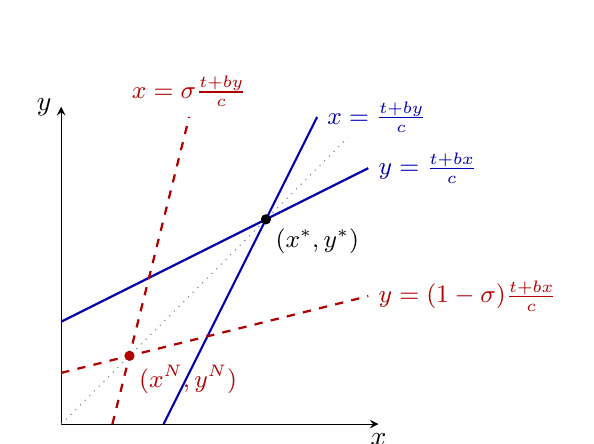
\begin{tikzpicture}[scale=2.6,>=stealth]
  \draw[->] (0,0) -- (1.55,0) node[below] {$x$};
  \draw[->] (0,0) -- (0,1.55) node[left] {$y$};
  \draw[thick,blue!70!black] (0.5,0) -- (1.25,1.5) node[right] {\small $x=\frac{t+by}{c}$};
  \draw[thick,blue!70!black] (0,0.5) -- (1.5,1.25) node[right] {\small $y=\frac{t+bx}{c}$};
  \draw[thick,red!70!black,dashed] (0.25,0) -- (0.625,1.5) node[above] {\small $x=\sigma\frac{t+by}{c}$};
  \draw[thick,red!70!black,dashed] (0,0.25) -- (1.5,0.625) node[right] {\small $y=(1-\sigma)\frac{t+bx}{c}$};
  \draw[dotted,gray] (0,0) -- (1.4,1.4);
  \fill (1,1) circle (0.025) node[below right] {\small $(x^*,y^*)$};
  \fill[red!70!black] (0.3333,0.3333) circle (0.025) node[below right] {\small $(x^N,y^N)$};
\end{tikzpicture}
\end{center}
\refbib{M\&R Ch.~2, p.~39 (transfers); Ch.~4, p.~108.}
\rubrica{
\item Both best replies: 0.75 pt. Equilibrium and uniqueness (slope product $<1$): 0.75 pt.
\item Impossibility proved from the FOCs at $(x^*,y^*)$: 0.75 pt (``by symmetry $\sigma=\frac12$ works'': 0 for that line).
\item Graph: axes and four labelled lines 0.4, both intersections on the diagonal in the right order 0.35.
}
\end{sol}

\textbf{d)} (3 points) At $\sigma=\tfrac12$, find in closed form the efficiency loss
$L=W^*-W(x^N,y^N)$ and the relative loss $L/W^*$. Prove that the relative loss is increasing in
$b$ and find its limits as $b\to0$ and $b\to c$.
\resolespaco
\begin{sol}
\passo{equilibrium value}{$x^N=y^N=t/(2c-b)$; on the diagonal $W(z,z)=2tz-(c-b)z^2$, so
$W^N=\dfrac{2t^2}{2c-b}-\dfrac{(c-b)t^2}{(2c-b)^2}=\dfrac{t^2(3c-b)}{(2c-b)^2}$.}
\passo{loss}{$L=\dfrac{t^2}{c-b}-\dfrac{t^2(3c-b)}{(2c-b)^2}
=\dfrac{t^2\,[(2c-b)^2-(3c-b)(c-b)]}{(c-b)(2c-b)^2}=\dfrac{t^2c^2}{(c-b)(2c-b)^2}$.}
\passo{relative loss}{$\dfrac{L}{W^*}=\dfrac{c^2}{(2c-b)^2}$, with
$\dfrac{\partial}{\partial b}\dfrac{L}{W^*}=\dfrac{2c^2}{(2c-b)^3}>0$. Limits: $b\to0$: $\tfrac14$;
$b\to c$: $1$. Also $x^N/x^*=(c-b)/(2c-b)$, from $\tfrac12$ to $0$.}
\intuicao{Without complementarity, halving each party's marginal revenue halves each investment
and costs a quarter of the value. With complementarity, each party's under-investment lowers the
other's return as well: the shortfall feeds on itself, and as $b\to c$ almost the whole value of
the system is lost. Aula 1's multiplier, working in reverse.}
\refbib{M\&R Ch.~4, p.~108, n.~8; Ch.~2, p.~39.}
\rubrica{
\item $W^N$: 1 pt. $L$ simplified: 1 pt. $L/W^*$, its monotonicity and both limits: 1 pt.
\item Arithmetic slip with the right method: $-0.5$ pt. Loss computed at $b=0$ only: max.\ 1 pt.
}
\end{sol}

\textbf{e)} (3 points) Parameter analysis. Prove the signs of the effects of $t$, $b$, $c$,
$\delta_A$, $\delta_S$ on $x^*$, $W^*$, $A$'s share $s_A$ and payoff in regime I, and the relative
loss $L/W^*$ in regime II at $\sigma=\tfrac12$. Tabulate them, study $\delta_A=\delta_S=\delta\to1$,
$\delta_S\to0$ and $b\to c$, and explain why the choice between regimes matters more when the
investments are strong complements.
\resolespaco
\begin{sol}
\passo{levels}{$x^*=t/(c-b)$, $W^*=t^2/(c-b)$: $+t$, $+b$, $-c$; no $\delta$.}
\passo{share}{$s_A=\dfrac{1-\delta_S}{1-\delta_A\delta_S}$:
$\partial_{\delta_A}s_A=\dfrac{\delta_S(1-\delta_S)}{(1-\delta_A\delta_S)^2}>0$,
$\partial_{\delta_S}s_A=-\dfrac{1-\delta_A}{(1-\delta_A\delta_S)^2}<0$; independent of $t,b,c$.
Payoff $s_AW^*$ combines both.}
\passo{relative loss}{$L/W^*=c^2/(2c-b)^2$: $+b$ (item d); $\partial_c=-2bc/(2c-b)^3<0$; no
$t$, no $\delta$.}
\begin{center}
\begin{tabular}{lccccc}\toprule
 & $t$ & $b$ & $c$ & $\delta_A$ & $\delta_S$\\\midrule
$x^*$, $W^*$ & $+$ & $+$ & $-$ & $0$ & $0$\\
$s_A$ & $0$ & $0$ & $0$ & $+$ & $-$\\
$A$'s payoff $s_AW^*$ & $+$ & $+$ & $-$ & $+$ & $-$\\
$L/W^*$ (regime II) & $0$ & $+$ & $-$ & $0$ & $0$\\\bottomrule
\end{tabular}
\end{center}
\passo{limits}{$\delta_A=\delta_S=\delta\to1$: $s_A=1/(1+\delta)\to\tfrac12$, the first-mover
advantage vanishes. $\delta_S\to0$: $s_A\to1$ ($S$ cannot wait). $b\to c$: $W^*\to\infty$ while
$L/W^*\to1$.}
\passo{reading}{In regime I the split (patience) and the system (complementarity) are separable:
the parties always build $(x^*,y^*)$. Regime II removes the transfers that the value
maximization principle needs (M\&R p.~39), so the split becomes the incentive and the incentive
becomes the system. The stronger the complementarity, the larger both the prize of regime I
($W^*$) and the share of it that regime II throws away: firms with tightly interlocking
investments have the most to gain from organizing the relationship so that the investments
themselves can be contracted on and paid for.}
\rubrica{
\item Signs of $x^*$, $W^*$, $s_A$ proved: 1 pt. Sign of $L/W^*$ in $c$: 0.5 pt.
\item Table: 0.25 pt; limits: 0.5 pt; reading linking transfers, complementarity and regime choice: 0.75 pt.
\item Cross-topic reading missing (answer stays inside one model): max.\ half the item.
}
\end{sol}

\end{document}
